\section{Appendix: MVA Outputs}
\label{app:mvaoutputs}

The classifier outputs after MVA training for the likelihood discriminant 
are shown in Figs~\ref{fig:outputs170to300mu}--\ref{fig:outputs350to600mu}
for all Higgs mass points, muon category.
%%%%%%%%%%%%%%%%%%%
\begin{figure}[ht]
  \subfigure[$M_H$=170~GeV]{
    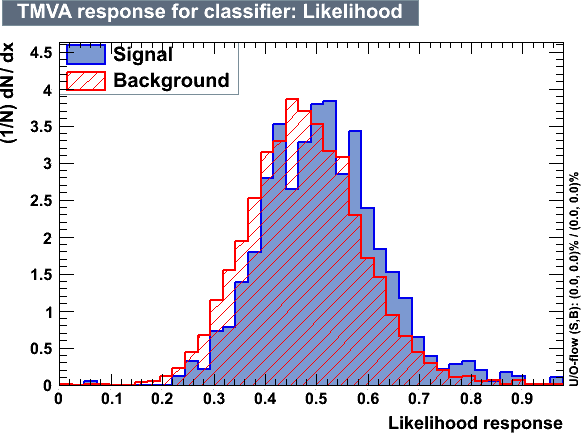
\includegraphics[width=0.42\textwidth]{plots/2012_MVA/TMVA_170_nJ2_mu_mva_Likelihood}	
  }
  \hspace{1cm}
  \subfigure[$M_H$=180~GeV]{
    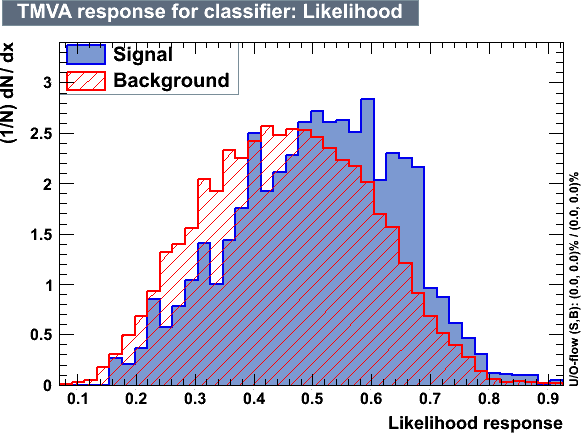
\includegraphics[width=0.42\textwidth]{plots/2012_MVA/TMVA_180_nJ2_mu_mva_Likelihood}
  }
  \\
  \subfigure[$M_H$=190~GeV]{
    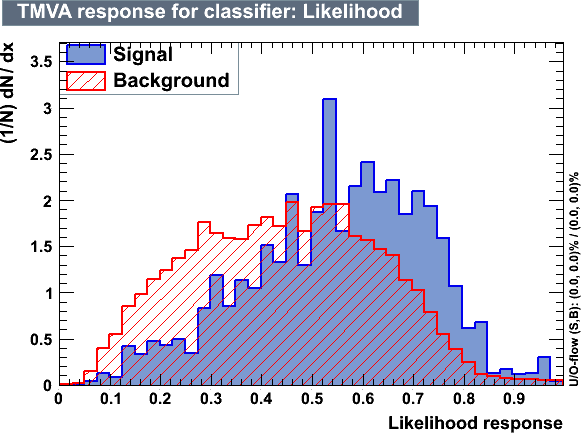
\includegraphics[width=0.42\textwidth]{plots/2012_MVA/TMVA_190_nJ2_mu_mva_Likelihood}
  }
  \hspace{1cm}
  \subfigure[$M_H$=200~GeV]{
    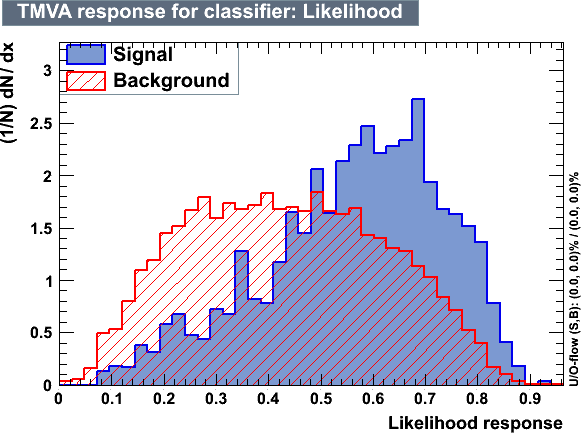
\includegraphics[width=0.42\textwidth]{plots/2012_MVA/TMVA_200_nJ2_mu_mva_Likelihood}
  }
  \\
  \subfigure[$M_H$=250~GeV]{
    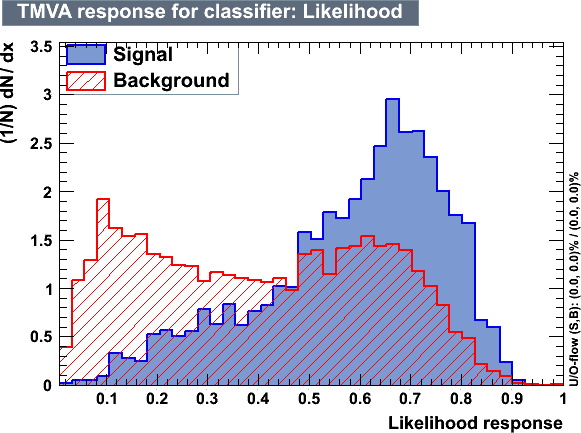
\includegraphics[width=0.42\textwidth]{plots/2012_MVA/TMVA_250_nJ2_mu_mva_Likelihood}
  }
  \hspace{1cm}
  \subfigure[$M_H$=300~GeV]{
    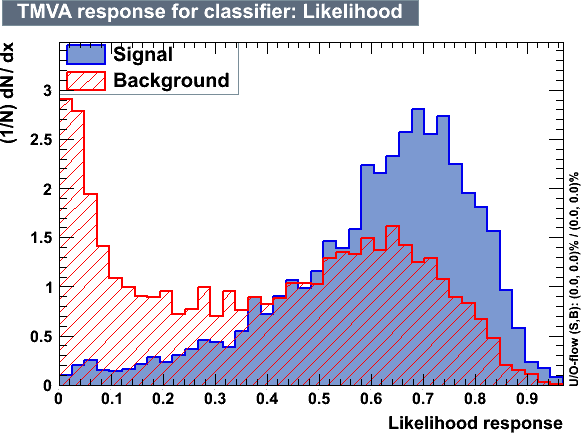
\includegraphics[width=0.42\textwidth]{plots/2012_MVA/TMVA_300_nJ2_mu_mva_Likelihood}
  }
  \caption{\label{fig:outputs170to300mu}Output of the multivariate discriminant for $M_H =$170--300~GeV , muon category}
\end{figure}
%%%%%%%%%%%%%%%%%%%
\newpage
%%%%%%%%%%%%%%%%%%%
\begin{figure}[ht]
  \subfigure[$M_H$=350~GeV]{
    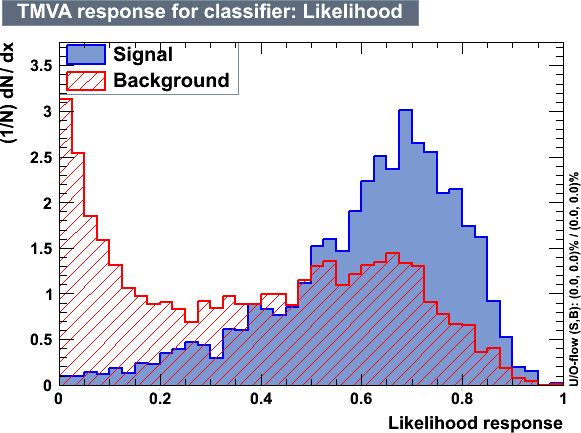
\includegraphics[width=0.42\textwidth]{plots/2012_MVA/TMVA_350_nJ2_mu_mva_Likelihood}
  }
  \hspace{1cm}
  \subfigure[$M_H$=400~GeV]{
    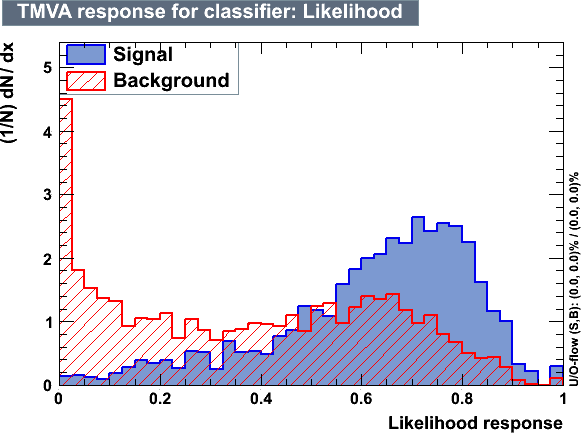
\includegraphics[width=0.42\textwidth]{plots/2012_MVA/TMVA_400_nJ2_mu_mva_Likelihood}
  }
  \\
  \subfigure[$M_H$=450~GeV]{
    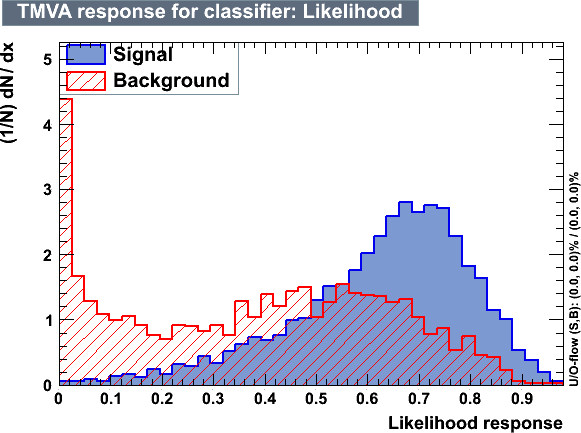
\includegraphics[width=0.42\textwidth]{plots/2012_MVA/TMVA_450_nJ2_mu_mva_Likelihood}
  }
  \hspace{1cm}
  \subfigure[$M_H$=500~GeV]{
    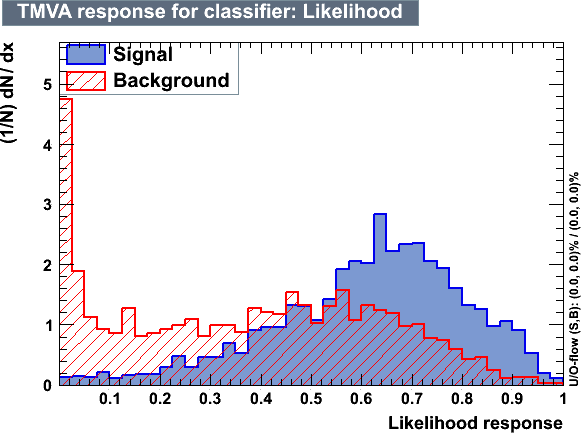
\includegraphics[width=0.42\textwidth]{plots/2012_MVA/TMVA_500_nJ2_mu_mva_Likelihood}
  }
  \\
  \subfigure[$M_H$=550~GeV]{
    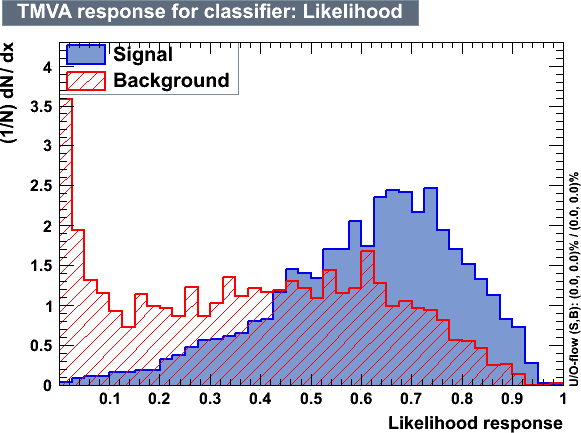
\includegraphics[width=0.42\textwidth]{plots/2012_MVA/TMVA_550_nJ2_mu_mva_Likelihood}
  }
  \hspace{1cm}
  \subfigure[$M_H$=600~GeV]{
    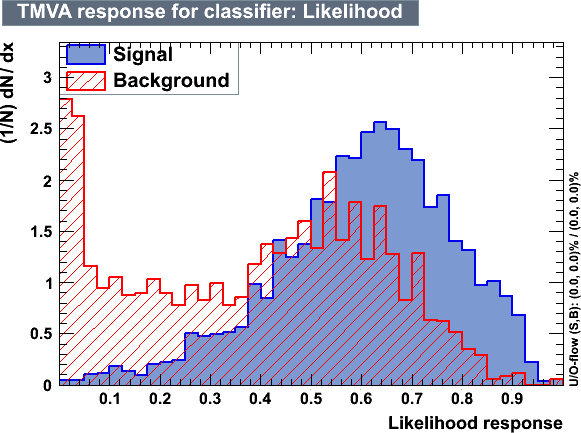
\includegraphics[width=0.42\textwidth]{plots/2012_MVA/TMVA_600_nJ2_mu_mva_Likelihood}
  }
  \caption{\label{fig:outputs350to600mu}Output of the multivariate discriminant for $M_H =$350--600~GeV , muon category}
\end{figure}
%%%%%%%%%%%%%%%%%%%
%%%%%%%%%%%%%%%%%%%
